\documentclass[10pt,apjl]{emulateapj}
\usepackage{amssymb} % for resolution symbol

\begin{document}

\shorttitle{Chemistry of the Orphan Stream I}
\shortauthors{Casey et al}


\title{Chemistry of the Orphan Stream I: Identifying Stream Members \\ from Low-Resolution Spectroscopy}

\author{Andrew R. Casey\altaffilmark{1,2}, Stefan C. Keller\altaffilmark{1}, Gary Da Costa\altaffilmark{1}, Elizabeth Maunder\altaffilmark{1}}
\altaffiltext{1}{Research School of Astronomy \& Astrophysics, Australian National University, Mount Stromlo Observatory, via Cotter Rd, Weston, ACT 2611, Australia; \email{acasey@mso.anu.edu.au}}
\altaffiltext{2}{Kavli Institute for Astrophysics and Space Research, Massachusetts Institute of Technology, 77 Massachusetts Avenue, Cambridge, MA 02139, USA}

\begin{abstract}
We present coordinates and properties of candidate K giant members in the Orphan Stream, which have been identified from low-resolution spectroscopic data taken with AAOmega on the Anglo-Australian Telescope. From modest S/N spectra and independent cuts in photometry, kinematics, gravity and metallicity we yield self-consistent, highly probable stream members. We find a revised stream distance of $22.5\,\pm\,1.0$\,kpc near the celestial equator, and our kinematic signature peaks at $V_{GSR} = 82.1\,\pm\,1.4$\,km s$^{-1}$. The observed velocity dispersion of our most probable members is consistent with arising from the velocity uncertainties alone. This indicates that at least along the line-of-sight, the Orphan Stream is kinematically quite cold. Our data indicates an overall stream metallicity of [Fe/H] $= -1.63\,\pm\,0.19$\,dex which is more metal-rich than previously found and unbiased by spectral type. Furthermore, the significant metallicity dispersion displayed by our probable members, $\sigma = 0.56$\,dex, suggests that the unidentified Orphan Stream parent is a dSph satellite. We highlight likely members for high-resolution spectroscopic follow-up.
\end{abstract}

\keywords{Galaxy: halo, structure --- Individual: Orphan Stream --- Stars: K-giants}

\section{Introduction}
\label{sec:introduction}

The Milky Way stellar halo has partly formed through the accretion of satellites which are disrupted by tidal forces as they fall into the Milky Way's potential. Stars which were once gravitationally bound to the satellite are left behind in a stream of stars. Stream kinematics are sensitive to the shape of the galactic potential, allowing us to constrain the Milky Way potential, and reconstruct the formation history of the Galaxy. The level of accreted substructure in the Milky Way has only recently become apparent through multi-band photometric surveys like the Sloan Digital Sky Survey (SDSS). The more prominent of the detectable substructures, like Sagittarius, have been well-studied. One of the more prominent \--- yet less studied \--- substructures is that of the Orphan Stream. 

The Orphan Stream was independently detected by both \citet{Grillmair_Dionatos_2006} and \citet{Belokurov_et-al_2006}, and is distinct from other substructures in the halo. The stream stretches over $60\,^\circ$ in the sky, has a low surface brightness and a narrow stream width of only $\sim$2\,$^\circ$ and as the name suggests, the parent object largely remains a mystery. The stream extends past the celestial equator \--- outside the SDSS footprint \--- but has not been detected in existing southern surveys \citep{Newberg_et-al_2010}. Whilst the parent system remains elusive, significant effort has been placed on associating the stream with known Milky Way satellites \citep{Zucker_et-al_2006, Fellhaur_et-al_2007,Jin_Lynden_Bell_2007,Sales_et-al_2008}. In contrast, there has been relatively limited observational work on the Orphan Stream itself other than the original discovery papers \citep{Grillmair_Dionatos_2006, Belokurov_et-al_2006, Belokurov_et-al_2007} and the work of \citet{Newberg_et-al_2010}. This is largely to be expected given the absence of multi-band photometry in the southern sky and the low total luminosity of the stream, making it difficult to reliably separate Orphan Stream members from halo stars. Further understanding on the extent of the stream awaits the SkyMapper and Pan-STARRS photometric surveys \citep{Keller_et-al_2007, Hodapp_et-al_2004}.

As \citet{Sales_et-al_2008} point out, there is a natural observational bias towards more massive and recent mergers like Sagittarius. Consequently, the fainter end of this substructure distribution has yet to be fully recovered, or thoroughly examined. Interestingly, there are indications that  some fainter substructures like the Orphan Stream and the Palomar 5 tidal tails \citep{Odenkirchen_et-al_2009} have orbits which seem to be best-fit by Milky Way models with nearly 60\% less mass \citep{Newberg_et-al_2010} than generally reported by \citet{Xue_et-al_2008} and \citet{Koposov_et-al_2010}. Such a discrepancy in the mass of the Milky Way is troublesome. More complete photometric and kinematic maps of these low total luminosity streams may provide the best test as to whether this mass discrepancy is real, or an artefact of incomplete observations. Whilst the full spatial extent of the Orphan Stream remains incomplete, we can examine the detailed chemistry of its members and investigate the stream history, as well as make predictions about the nature of the host system.

In this letter we present a detailed, self-consistent analysis to identify K giant members of the Orphan Stream. Using our selection method we have catalogued the locations of nine highly probable Orphan Stream candidates, all worthy of high-resolution spectroscopic follow up. In the following section we outline our photometric target selection. In \S\ref{sec:observations} we describe the low-resolution spectroscopic observations. The data analysis, including stream identification, is discussed in \S\ref{sec:analysis} and in \S\ref{sec:conclusions} the conclusions, predictions and future work are presented.


\section{Target Selection}
\label{sec:target-selection}

We have targeted K giant members of the Orphan Stream in order to investigate their detailed chemistry. Because K-giants are difficult to unambiguously detect from photometry alone, low-resolution spectroscopy is required to estimate stellar parameters and determine radial velocities. The Orphan Stream has a low spatial over-density on the order of $\sim$10\%, which makes it difficult to separate stream members from halo stars. However, there is a well described distance gradient along the stream \citep{Belokurov_et-al_2007, Newberg_et-al_2010} which provides an indication on where we should focus our spectroscopic efforts.

The Orphan Stream is closest to us in two locations on the edge of the SDSS footprint: at the celestial equator \citep{Belokurov_et-al_2007}, and along outrigger SEGUE Stripe 1540 \citep{Newberg_et-al_2010}. These two locations are unequivocally the best place to recover bright stream members. We have targeted two fields centered on $(\alpha, \delta) =$ (10:48:15, 00:00:00) and (10:48:15, $-$02:30:00), and employed a combination of colour cuts with the SDSS DR 7 \citep{Abazajian_et-al_2009} data set in order to identify likely K giants:
\begin{eqnarray}
0.6 <& (g-i)_0 &< 1.7 \\
-15(g-i)_0 + 27 <& g_0 &< -3.75(g-i)_0 + 22.5 \\
15  <& i_0  &< 18 
\end{eqnarray}

Given our colour selection we expect to recover giants, and dwarf contaminants. The lack of 2MASS photometry for the selected stars means we cannot use the $(J-H, H-K)$ diagram to aid the separation of candidate giants from contaminating dwarfs.

\section{Observations}
\label{sec:observations}

Observations took place on the Anglo-Australian Telescope using the AAOmega spectrograph in April 2009. AAOmega is a fibre-fed, dual beam multi-object spectrograph which is capable of simultaneously observing spectra of 392 (science and sky) targets across a $2\,^\circ$ field of view. We used the 5700\,{\AA} dichroic in combination with the 1000I grating in the red arm, and the 580V grating in the blue arm. This provides a spectral coverage between $800 \leq \lambda \leq 950$\,nm in the red at $\mathcal{R} \approx 4400$, and between $370 \leq \lambda \leq 580$\,nm with a lower resolving power of $\mathcal{R} \approx 1300$ in the blue.

The data were reduced using the standard \textsc{2DFDR} reduction pipeline\footnote{http://www.aao.gov.au/2df/aaomega/aaomega\_2dfdr.html}. After flat-fielding, throughput calibration for each fibre was achieved using the intensity of skylines in each fibre. The median flux of dedicated sky fibres was taken for sky subtraction, and wavelength calibration was performed using arc lamp exposures between science frames. Three thirty minute science exposures were median combined to assist with cosmic ray removal. The median S/N obtained in the red arm for our fields is modest at 35 per pixel. With the presence of strong Ca\,\textsc{II} triplet lines in the red arm we are able to ascertain reliable radial velocities and reasonable estimates on overall metallicity \citep[][and references therein]{Starkenburg_et-al_2010}. Our spectral region also includes gravity-sensitive magnesium lines: Mg\,\textsc{I} at 8807\,{\AA}, and the Mg\,\textsc{I}\,b 3$p$-4$s$ triplet lines at $\sim$5178\,{\AA}. As we demonstrate in the next section, these lines are sufficient to discriminate dwarfs from giants even with weak signal.

The blue and red arm spectra were normalised using a third order cubic spline after multiple iterations of outlier clipping. We used defined knot spacings of 20 nm in the red arm, and 5 nm in the blue arm in order to accommodate often poor S/N, and varying strengths of molecular band-heads.

\section{Analysis}
\label{sec:analysis}

We have employed a combination of separate criterion to identify likely Orphan Stream members: kinematics, a giant/dwarf indication from Mg\,\textsc{I} lines, and consistent metallicities from isochrone fitting and the Ca\,\textsc{II} triplet lines. Each criterion is discussed here separately.

\subsection{Kinematics}
Radial velocities were measured by cross-correlating our normalised spectra against a K-giant synthetic template with a temperature of 4500\,K, $\log{g}$ = 1 and $[\mbox{Fe/H}] = -1.5$ across the range $845 \leq \lambda \leq 870$\,nm. Heliocentric velocities were translated to the galactic rest frame by adopting the local standard of rest velocity as 220\,km s$^{-1}$ towards $(l, b) = (53\,^\circ, 25\,^\circ)$ \citep{Kerr_Lynden-Bell_1986, Mihalas_Binney_1981}\footnote{Where $V_{GSR} = V_{\textsc{helio}} + 220\sin{l}\cos{b} + 16.5\times[\sin{b}\sin{25} + \cos{b}\cos{25}\cos{(l - 53)}]$}. \citet{Newberg_et-al_2010} presented a comprehensive kinematic dataset on the Orphan Stream using BHB stars and employed a slightly different galactocentric transformation. This systematic difference equates to our galactocentric rest frame velocities being on average $\sim$5\,km s$^{-1}$ lower than those of \citet{Newberg_et-al_2010}.

\begin{figure}[h]
	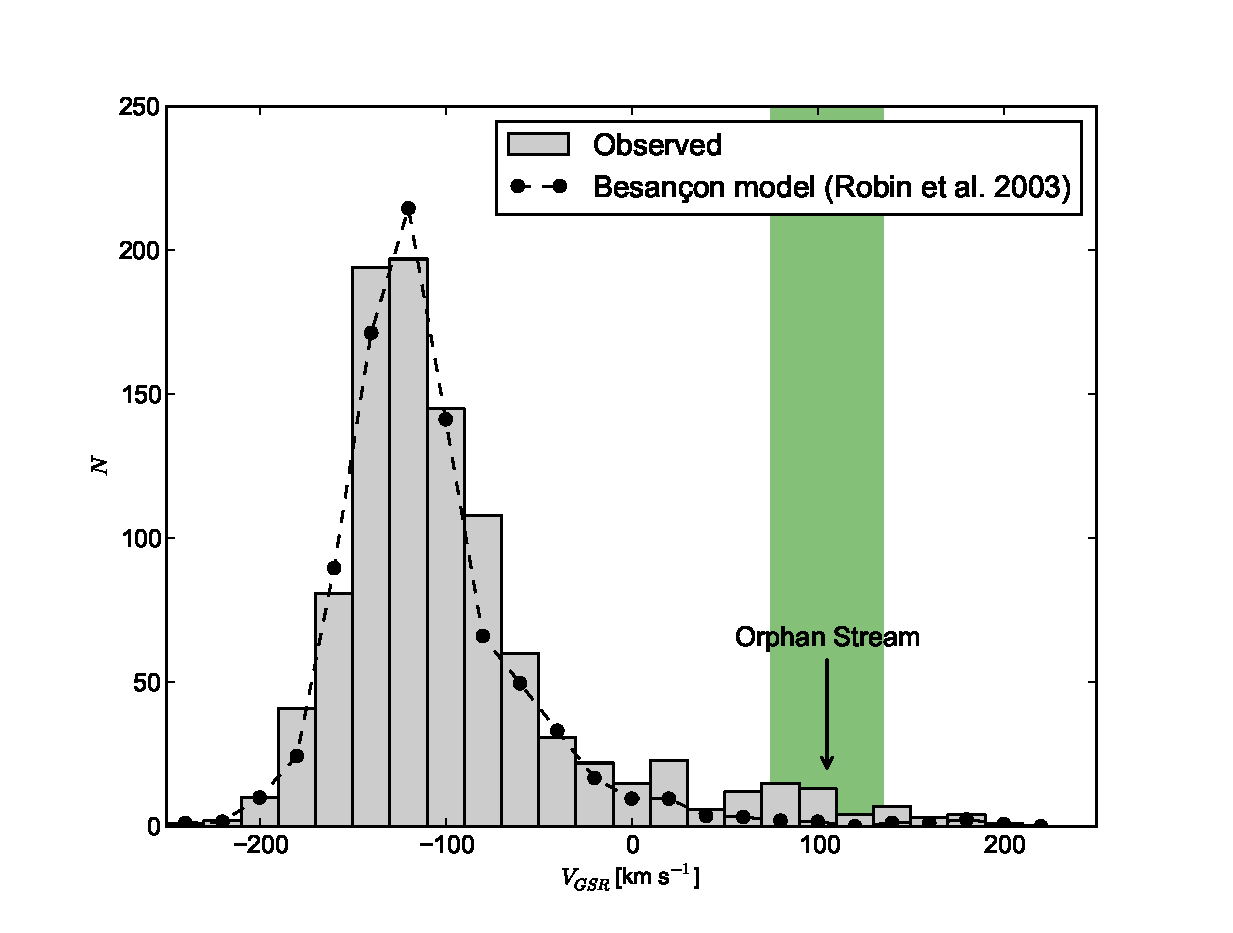
\includegraphics[width=\columnwidth]{./fig1.eps}
	\caption{Galactocentric rest frame velocities for stars in both our observed fields (grey), and predicted Besan\c{c}on velocities which have been scaled to match our observed sample size. The expected kinematic signature from \citet{Newberg_et-al_2010} for the Orphan Stream is highlighted, as is our kinematic selection window (green).}
	\label{fig:velocities}
\end{figure}

Figure \ref{fig:velocities} shows a histogram of our galactocentric velocities, compared to the predicted smooth line-of-sight velocity distribution for this region from the Besan\c{c}on model \citep{Robin_et-al_2003}. We have selected predicted stars from the Besan\c{c}on model using the same criterion as outlined in \S\ref{sec:target-selection} after using the \citet{Jordi_et-al_2006} colour transformations. It is clear that our target selection has yielded mostly nearby thick disk dwarf stars with $V_{GSR} \approx -120$\,km s$^{-1}$. The expected kinematic signature for the Orphan Stream, as \citet{Newberg_et-al_2010} reported, is labelled in Figure \ref{fig:velocities}. There is no obvious sharp kinematic peak representative of the Orphan Stream in our sample. From kinematics alone, our targets appears largely indistinguishable from a smooth halo distribution.

In this region \citet{Newberg_et-al_2010} found the Orphan Stream to have $V_{GSR} = 110$ km s$^{-1}$ from BHB stars, approximately $105$\,km s$^{-1}$ on our scale. To isolate potential Orphan Stream members we have nominated a relatively wide kinematic selection region between $75 \leq V_{GSR} \leq 135$ km s$^{-1}$, which yields twenty-five Orphan Stream candidates. The typical uncertainty in our velocities is $\pm{}5.0$\,km s$^{-1}$, although for our fainter targets this quickly increases above 10\,km s$^{-1}$.

\subsection{Dwarf/Giant Discrimination}
\label{sec:dwarf-giant}

We have measured the equivalent width of the gravity-sensitive Mg\,\textsc{I} line at 8807 \AA{} to distinguish dwarfs from giants \citep{Battaglia_Starkenburg_2012}. At a given temperature (or $g - r$) and metallicity, giant stars present narrower Mg\,\textsc{I} absorption lines than their dwarf contaminants. Given our target selection, our sample is likely to contain many more dwarfs than giants. In some cases no Mg\,\textsc{I} 8807 \AA{} line was apparent, so an upper limit was estimated based on the S/N. In these cases the candidate was considered a ``non-dwarf" because we cannot exclusively rule out a metal-poor sub-giant with this criterion alone. For these purposes we are only looking for a simple indication as to whether a star is likely a dwarf or not. Figure \ref{fig:ew-mg} illustrates the trend with EW$_{\lambda8807}$ against SDSS de-reddened\footnote{All magnitudes presented in this letter are de-reddened using the \citet{Schlegel_Finkbeiner_Davis_1998} dust maps.} $g - r$, illustrating the dominant upper dwarf branch we wish to exclude. The adopted dwarf/giant separation line is shown. Admittedly this selection criterion is not particularly strict, but we are allowing multiple inclusive cuts and taking the intersection of these criteria to identify Orphan Stream giants.

\begin{figure}[h]
	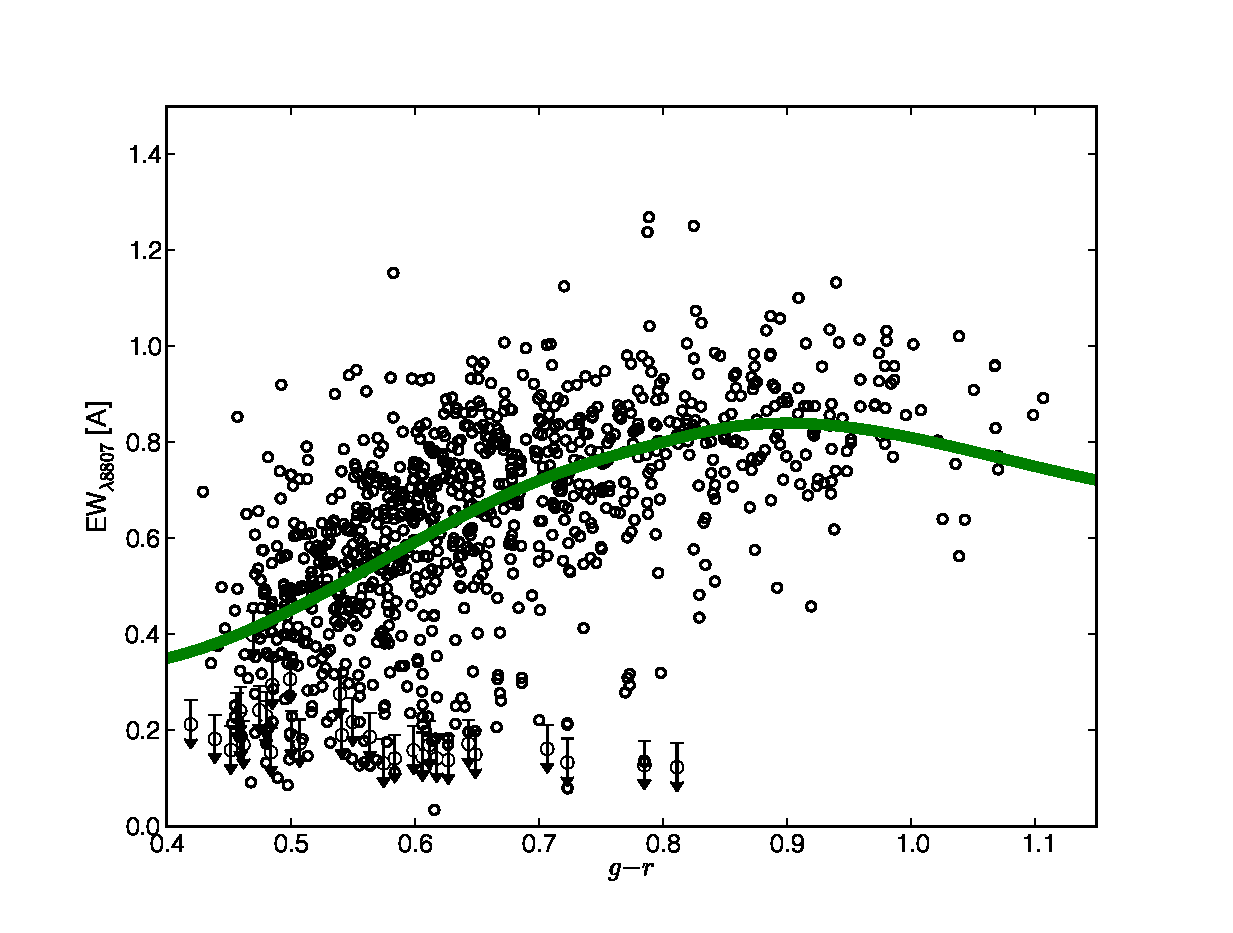
\includegraphics[width=\columnwidth]{./fig2.eps}
	\caption{SDSS $g - r$ against the measured equivalent width of the Mg\,\textsc{I} transition at 8807\,\AA{}. Dwarf contaminants occupy the more populous upper branch. Our separation line between dwarfs and giants is shown in green.}
	\label{fig:ew-mg}
\end{figure}

This analysis was also performed using the total equivalent width of the Mg\,\textsc{I}\,b triplet lines. Both analyses were entirely consistent with each other: essentially the same candidate selection was found using both techniques. However, given slightly poorer signal at the Mg\,\textsc{I}\,b triplet, we were forced to adopt many more upper limits than when using the 8807\,{\AA} line. Because we classify all upper limits as being ``non-dwarfs" (i.e. potential OSS giants), we deduced a slightly larger candidate sample for the Mg\,\textsc{I}\,b analysis, which was primarily populated by upper limits. In conclusion, we found the Mg\,\textsc{I} line at 8807\,{\AA} appeared to be a more consistent dwarf discriminant given our weak S/N \--- particularly for our fainter stars \--- and thus we have used the 8807\,{\AA} Mg\,\textsc{I} selection throughout the rest of our analysis.

Our dwarf/giant separation line in Figure \ref{fig:ew-mg} yields 425 potential giants. This fraction of giants ($\sim$44\%) is much larger than what would be expected given our selection criterion (e.g. see \citeauthor{Casey_et-al_2012} \citeyear{Casey_et-al_2012}a). Hence, our gravity criterion is extremely inclusive and susceptible to dwarf contamination. Upon taking the intersection of our kinematic and gravity selections, we deduce eighteen stars that appear likely Orphan Stream K giants.


\subsection{Metallicities}
\label{sec:metallicities}

We have measured the equivalent widths of the Ca\,\textsc{II} near-infrared triplet lines for stars that meet our kinematic and surface gravity criteria. After correcting for luminosity, the equivalent width of the Ca\,\textsc{II} triplet lines provide a good indication of the overall metallicity of a RGB star \citep{Amandroff_Da_Costa_1991}. We have employed the \citet{Starkenburg_et-al_2010} relationship and corrected for luminosity in $g$ against the horizontal branch magnitude at $g_{HB}$ = 17.1 \citep{Newberg_et-al_2010}. Strictly speaking, the Ca\,\textsc{II}\---[Fe/H] calibration is only valid for stars brighter than the horizontal branch, although the relationship only becomes significantly inappropriate near $g \-- g_{HB} \sim +1$ \citep{Saviane_et-al_2012}. Many of our candidates are fainter than this valid luminosity range, and therefore they should not be excluded solely because of their derived metallicities. Stars fainted than $g_{HB}$ will have slightly lower metallicities than predicted by our Ca\,\textsc{II}\---[Fe/H] relationship, and for these stars we will only use metallicities to assign a relative qualitative likelihood for stream membership.
Given a distance to the Orphan Stream, we can also estimate a star's metallicity through isochrone fitting. We have used a 10\,Gyr \citet{Girardi_et-al_2008} isochrone at 21.4\,kpc \citep{Newberg_et-al_2010} and found metallicities for all eighteen likely stream members from their best-fitting isochrone. Derived metallicities from Ca\,\textsc{II} line strengths and isochrone fitting that are consistent (within $\pm0.3$\,dex) indicates these measurements are reliable, and that these stars are indeed at a distance of $\sim$21.4\,kpc. We find ten highly likely stream members with consistently derived metallicities. They fall within the shaded region illustrated in Figure \ref{fig:feh}. 


\begin{deluxetable*}{lccccccccccccc}
\tabletypesize{\scriptsize}
\tablecolumns{12}
\tablewidth{0pt}
\tablecaption{Identified Orphan Stream Candidates\label{tab:oss-members}}
\tablehead{
	\colhead{Star} &
	\colhead{$\alpha$} &
	\colhead{$\delta$} &
	\colhead{$g$} &
	\colhead{$g \-- r$} &
	\colhead{$\mu_{total}$\tablenotemark{a}} &
	\colhead{$V_{GSR}$} &
	\colhead{$EW_{\lambda8807}$} &
	\colhead{[Fe/H]$_{Ca}$} &
	\colhead{[Fe/H]$_{iso}$} &
	\colhead{[Fe/H]\tablenotemark{b}} &
	\colhead{Stream} \\
Name & (J2000) & (J2000) & & & (mas yr$^{-1}$) & (km s$^{-1}$) & (\AA) & (dex) & (dex) & (dex) & Prob.
}
\startdata
OSS-1  & 10:46:21.9 & $+$00:43:21.8 & 17.52 & 0.50 &\phn6.1 $\pm$ 6.1 & \phn73.3 $\pm$ \phn9.3 & 0.273 & --1.78 &$<$--2.28& --1.78 & Low \\
OSS-2  & 10:46:29.3 & $-$00:19:38.5 & 17.77 & 0.56 &\phn2.7 $\pm$ 6.1 & \phn78.4 $\pm$ \phn5.2 & 0.126 & --1.63 & --1.68  & --1.63 & High \\
OSS-3  & 10:46:50.4 & $-$00:13:15.6 & 17.33 & 0.51 &\phn5.9 $\pm$ 6.1 & \phn77.0 $\pm$ \phn4.0 & 0.416 & --1.31 &$<$--2.28& --1.31 & Low \\
OSS-4  & 10:47:06.1 & $-$01:56:03.9 & 18.74 & 0.54 &\phn7.8 $\pm$ 6.9 & \phn74.9 $\pm$    17.6 & 0.452 &:--1.12\tablenotemark{c}& --1.40  & --1.40 & High \\
OSS-5  & 10:47:15.0 & $-$03:15:03.9 & 18.66 & 0.54 &\phn8.4 $\pm$ 7.4 &    109.5 $\pm$ \phn9.0 &$<$0.19&:--1.85\tablenotemark{c}& --1.43  & --1.43 & Medium \\
OSS-6  & 10:47:17.6 & $+$00:25:07.7 & 16.09 & 0.72 &\phn0.8 $\pm$ 5.7 & \phn79.2 $\pm$ \phn3.3 & 0.212 & --1.84 & --1.80  & --1.84 & High \\
OSS-7  & 10:47:29.1 & $-$02:02:22.6 & 17.86 & 0.47 &     \nodata      & \phn93.2 $\pm$    29.8 &$<$0.40& --2.82 &$<$--2.28& --2.82 & High \\
OSS-8  & 10:47:30.1 & $-$00:01:24.5 & 17.25 & 0.61 &\phn6.6 $\pm$ 5.9 & \phn83.6 $\pm$ \phn3.5 & 0.123 & --1.62 & --1.68  & --1.62 & High \\
OSS-9  & 10:48:20.9 & $+$00:26:34.4 & 17.88 & 0.55 &\phn9.7 $\pm$ 6.1 &    118.9 $\pm$    11.7 & 0.467 & --1.65 & --1.73  & --1.65 & High \\
OSS-10 & 10:48:27.8 & $+$00:55:24.0 & 17.72 & 0.51 &   15.3 $\pm$ 6.5 &    124.5 $\pm$ \phn6.7 & 0.182 & --1.48 &$<$--2.28& --1.48 & Low \\
OSS-11 & 10:48:31.9 & $+$00:03:35.7 & 17.02 & 0.58 &\phn8.5 $\pm$ 5.8 &    105.1 $\pm$ \phn5.1 & 0.234 & --1.12 & --2.10  & --1.12 & Low \\
OSS-12 & 10:48:44.4 & $-$02:53:08.8 & 18.35 & 0.62 &\phn3.8 $\pm$ 6.6 &    108.2 $\pm$ \phn9.0 & 0.183 &:--1.01\tablenotemark{c}& --1.17  & --1.17 & High \\
OSS-13 & 10:48:46.9 & $-$00:32:27.8 & 17.85 & 0.46 &   30.9 $\pm$ 6.8 &    109.3 $\pm$ \phn8.1 & 0.324 & --2.37 &$<$--2.28& --2.37 & Medium \\
OSS-14 & 10:49:08.3 & $+$00:02:00.2 & 16.27 & 0.62 &\phn7.7 $\pm$ 5.7 & \phn81.5 $\pm$ \phn4.6 & 0.034 & --2.70 &$<$--2.28& --2.70 & High \\
OSS-15 & 10:50:13.1 & $+$00:33:52.7 & 16.13 & 0.58 &\phn8.4 $\pm$ 5.7 & \phn94.7 $\pm$ \phn5.1 & 0.391 & --1.54 &$<$--2.28& --1.54 & Low \\
OSS-16 & 10:50:24.2 & $-$01:49:05.4 & 17.94 & 0.54 &\phn4.0 $\pm$ 6.5 & 109.9    $\pm$    25.4 & 0.151 & --1.06 & --1.73  & --1.06 & Low \\
OSS-17 & 10:50:33.8 & $+$00:12:19.1 & 17.82 & 0.60 &\phn8.1 $\pm$ 7.1 & \phn97.5 $\pm$ \phn5.9 & 0.596 & --0.90 & --1.43  & --0.90 & Medium \\
OSS-18 & 10:51:19.7 & $+$00:05:15.5 & 17.81 & 0.65 &   12.5 $\pm$ 6.6 & \phn82.7 $\pm$ \phn5.0 & 0.198 & --1.16 & --1.20  & --1.16 & High 
\enddata
\tablenotetext{a}{Proper motions and uncertainties in $\alpha$ and $\delta$ added in quadrature.}
\tablenotetext{b}{Final adopted [Fe/H] value based on quality of two metallicity measurements.}
\tablenotetext{c}{Sufficiently fainter than $g_{HB}$ to qualify this measurement as uncertain.}
\end{deluxetable*}

\begin{figure}[h!]
	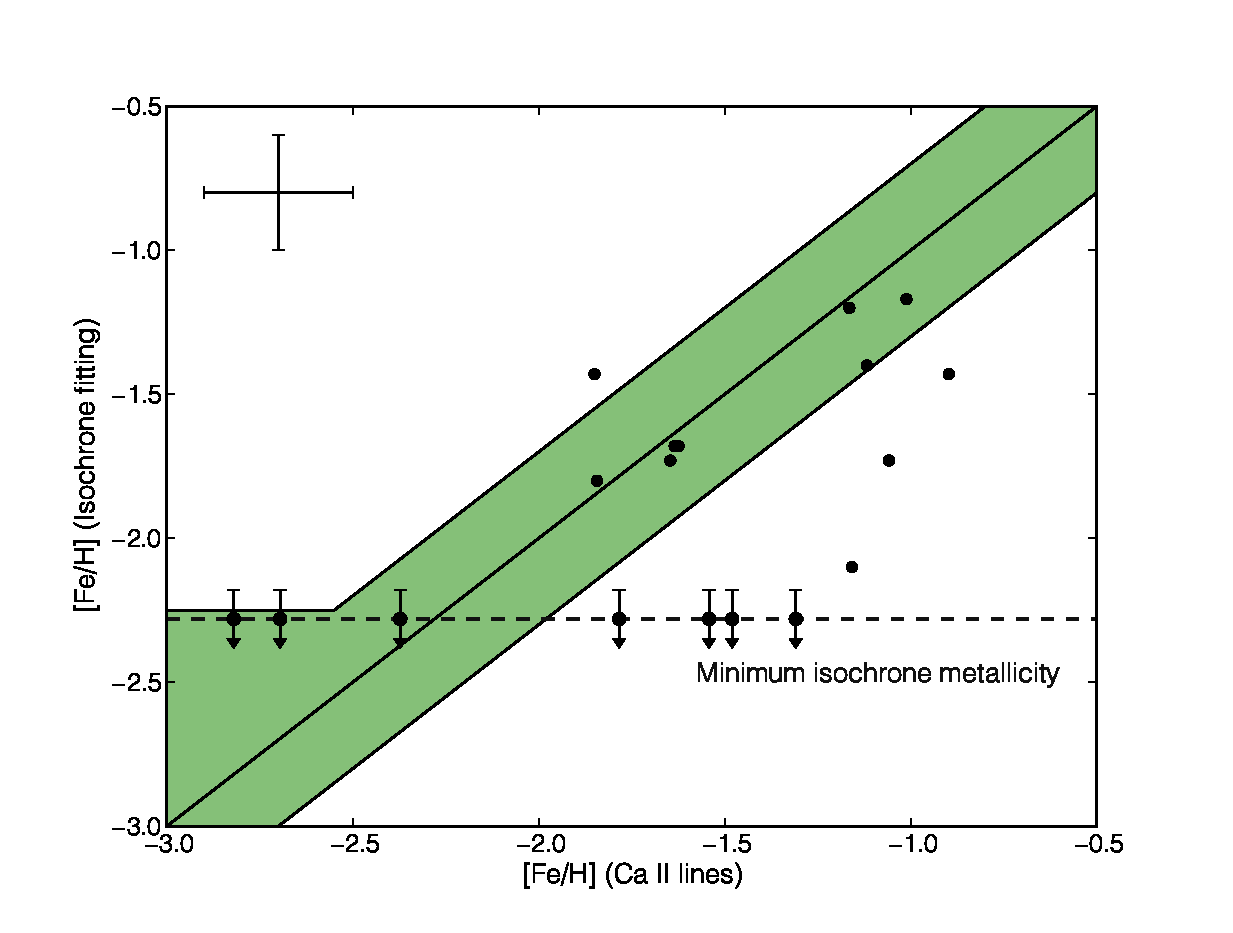
\includegraphics[width=\columnwidth]{./fig3.eps}
	\caption{Metallicities from the Ca\,\textsc{II} triplet lines versus those found from fitting isochrones to the eighteen stars that meet our kinematic and surface gravity criteria. Both abundance determinations imply these stars are RGB members of the Orphan Stream at a distance of $\sim$21.4\,kpc \citep{Newberg_et-al_2010}. Consistency between these methods indicates highly likely stream membership (green region). The minimum isochrone [Fe/H], and a representative uncertainty of 0.2\,dex for abundance measurements is shown.}
	\label{fig:feh}
\end{figure}

We have investigated the status of these ten stars in the PPMXL proper motion catalogue \citep{Roeser_et-al_2010}, finding entries for nine of the candidates. One star (OSS-13 in Table \ref{tab:oss-members}) has a listed proper motion that is different from that of the other nine members at the $6\,\sigma$ level. Consequently, we have reduced the membership likelihood of this star from ``High" to ``Medium".

We have adopted a final overall metallicity for each star based on the quality of our [Fe/H] measurements. Adopted values are tabulated in Table \ref{tab:oss-members}. From our nine highly likely stream members we find an overall stream metallicity of $[\mbox{Fe/H}] = -1.63$ with a dispersion of $\sigma = 0.56$ dex. This abundance spread is larger than typically seen in globular cluster stars and is more representative of the chemical spreads seen in dSph satellites. \citet{Newberg_et-al_2010} found a stream metallicity of $[\mbox{Fe/H}] = -2.1$ from BHB stars, which is not inconsistent with our measurement given the spread in Orphan Stream K-giant metallicities.

\begin{figure}[h!]
	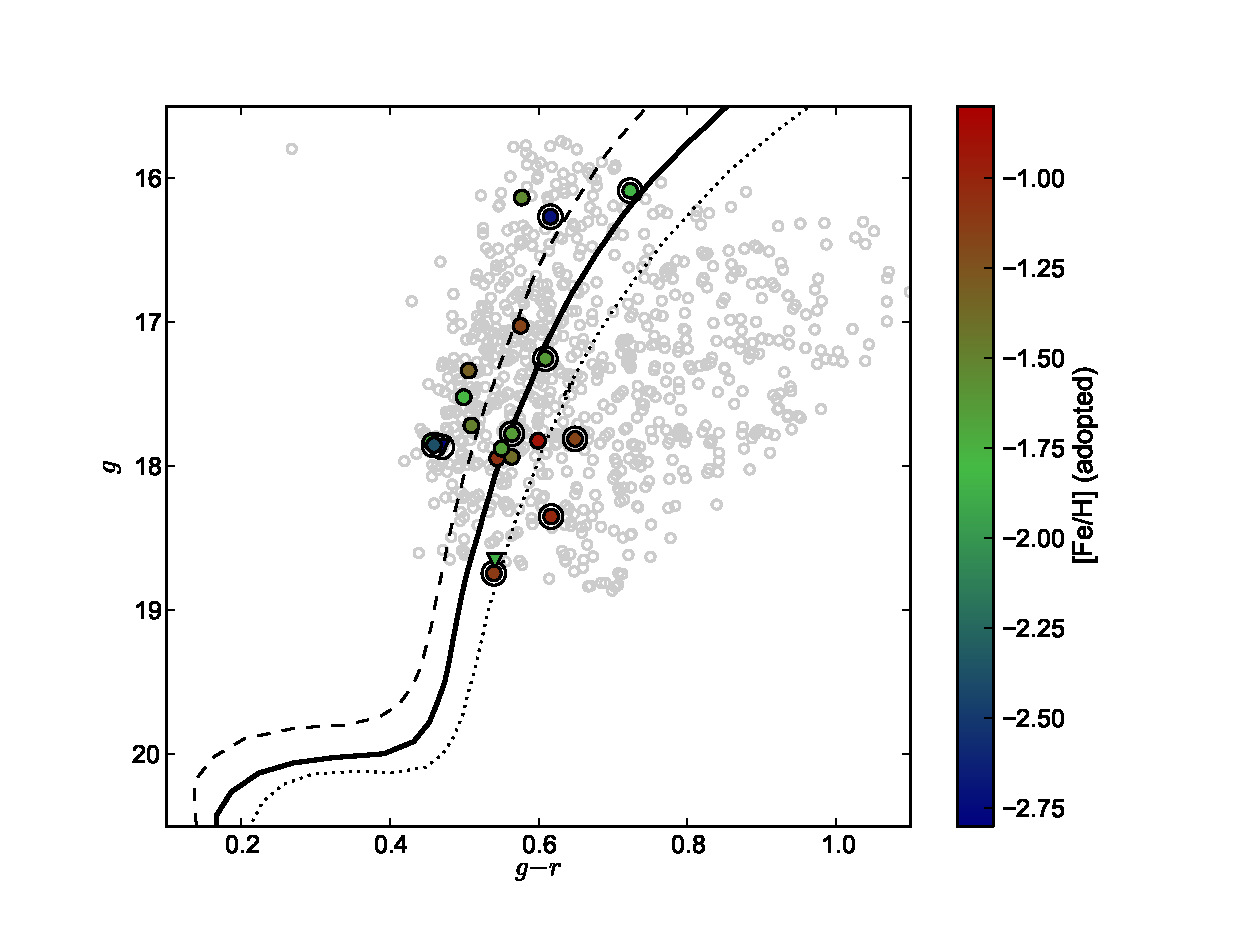
\includegraphics[width=\columnwidth]{./fig4.eps}
	\caption{Color magnitude diagram showing our observed candidates (grey). Observations fulfilling kinematic and gravity cuts are colored by their metallicity, and those with upper limits for surface gravity are marked as triangles ($\triangledown$). Highly probable stream members (see text) are circled. Relevant 10\,Gyr \citet{Girardi_et-al_2008} isochrones at $[\mbox{Fe/H}] = -1.5$ (dotted), $-2.0$ (dashed) at 21.4\,kpc \citep{Newberg_et-al_2010} are shown, as well as our best-fitting 10\,Gyr isochrone of $[\mbox{Fe/H}] = -1.63$ at 22.5\,kpc (solid).}
	\label{fig:cmd}
\end{figure}

Given that our Orphan Stream giants cover a wide evolutionary range along the giant branch (Figure \ref{fig:cmd}), we are in a good position to revise the distance estimate to the stream. Given a 10\,Gyr \citet{Girardi_et-al_2008} isochrone at $[\mbox{Fe/H}] = -1.63$, we find a best-fitting distance to the stream of $22.5 \pm 1.0$\,kpc at $(l, b) = (250\,^\circ,\,50\,^\circ)$. This isochrone is shown in Figure \ref{fig:cmd}, illustrating that three of our nine most probable member stars lie perfectly on this isochrone. Our derived distance is in reasonably good agreement with the $21.4 \pm 1.0$\,kpc deduced by \citet{Newberg_et-al_2010}.


\section{Conclusions}
\label{sec:conclusions}

We have presented a detailed analysis to isolate individual Orphan Stream K giants from low-resolution spectroscopy using a combination of photometric, kinematic, gravity, metallicity, and proper motion information. Although each individual criterion is likely to induce some level contamination, their intersection reveals nine highly probable, self-consistent, Orphan Stream K giants.  We deduce a median stream metallicity of $[\mbox{Fe/H}] = -1.63 \pm 0.19$ and find an intrinsically wide metallicity spread of $\sigma = 0.56$\,dex, indicative of a dSph origin. Unlike other stellar tracers, K-type giants can exist at all metallicities, hence our derived metallicity spread is likely representative of the true stream metallicity distribution function. Recall that the metallicity determination was performed after kinematic and gravity cuts, and three of our most probable members lay perfectly on a 10\,Gyr isochrone of $[\mbox{Fe/H}] = -1.63$. Our stream members indicate a distance to the stream of $22.5 \pm 1.0$\,kpc at $(l, b) = (250\,^\circ,\,50\,^\circ)$, in agreement with that deduced by \citet{Newberg_et-al_2010}.

If the Orphan Stream continues through SEGUE Stripe 1540 at $(l, b) = (271\,^\circ,\,38\,^\circ)$ as \citet{Newberg_et-al_2010} found, then the stream is even closer there than in the region analysed here. Thus, if our observations and analyses are repeated at $(271\,^\circ,\,38\,^\circ)$, we predict K giant stream members of brighter apparent magnitude will be recovered.

Using a maximum-likelihood estimation we find the stream velocity at $(l, b) = (250\,^\circ, 50\,^\circ)$ from nine stars to be $V_{GSR} = 85.3 \pm 4.4$\,km s$^{-1}$ and the dispersion to be $6.5 \pm 7.0$\,km s$^{-1}$. If we exclude three stars with weak signal \--- and hence large ($> 10$\,km s$^{-1}$) velocity uncertainties \--- the peak occurs at $82.1 \pm 1.4$\,km s$^{-1}$ and the intrinsic dispersion is found to be $0.2\,\pm\,3.1$\,km s$^{-1}$. Hence, the observed stream dispersion is dominated by the velocity uncertainties, indicating that the intrinsic dispersion is small. Finally, these velocities indicate that the Orphan Stream is a very cold stream, and implies their motion is largely perpendicular to the line of sight.

The K giants presented here can provide great insight into the chemistry, and history of the Orphan Stream. High-resolution spectroscopic observations have been taken for some of our most highly probable members and a detailed chemical analysis will be presented in a forthcoming paper (Casey et al. 2012c, in preparation). Detailed chemical abundances can help determine both the nature of the host system before it's discovered, and allows us to compare peculiar chemical signatures with those of the known Milky Way satellites in order to associate likely parents. However, at least for the moment, the Orphan Stream remains appropriately named.


\acknowledgements
ARC acknowledges the financial support through the Australian Research Council Laureate Fellowship 0992131, and from the Australian Prime Minister's Endeavour Award Research Fellowship, which has facilitated his research at MIT. SK and GDaC acknowledge the financial support from the Australian Research Council through Discovery Programs DP0878137 and DP120101237. GDaC is also grateful for the support received during an extended visit to the Institute of Astronomy, University of Cambridge, during which this work was completed.

Funding for the SDSS and SDSS-II has been provided by the Alfred P. Sloan Foundation, the Participating Institutions, the National Science Foundation, the U.S. Department of Energy, the National Aeronautics and Space Administration, the Japanese Monbukagakusho, the Max Planck Society, and the Higher Education Funding Council for England. The SDSS Web Site is http://www.sdss.org/.

The SDSS is managed by the Astrophysical Research Consortium for the Participating Institutions. The Participating Institutions are the American Museum of Natural History, Astrophysical Institute Potsdam, University of Basel, University of Cambridge, Case Western Reserve University, University of Chicago, Drexel University, Fermilab, the Institute for Advanced Study, the Japan Participation Group, Johns Hopkins University, the Joint Institute for Nuclear Astrophysics, the Kavli Institute for Particle Astrophysics and Cosmology, the Korean Scientist Group, the Chinese Academy of Sciences (LAMOST), Los Alamos National Laboratory, the Max-Planck-Institute for Astronomy (MPIA), the Max-Planck-Institute for Astrophysics (MPA), New Mexico State University, Ohio State University, University of Pittsburgh, University of Portsmouth, Princeton University, the United States Naval Observatory, and the University of Washington.

% Note to the reader:
% In the acknowledgements, the final line including the text "the University of Washington"
% line does not appear if I don't have \phn here.
\phn

\begin{thebibliography}{26}
\expandafter\ifx\csname natexlab\endcsname\relax\def\natexlab#1{#1}\fi

\bibitem[{{Abazajian} {et~al.}(2009){Abazajian}, {Adelman-McCarthy},
  {Ag{\"u}eros}, {Allam}, {Allende Prieto}, {An}, {Anderson}, {Anderson},
  {Annis}, {Bahcall}, \& et~al.}]{Abazajian_et-al_2009}
{Abazajian}, K.~N., {et~al.} 2009, \apjs, 182, 543

\bibitem[{{Armandroff} \& {Da Costa}(1991)}]{Amandroff_Da_Costa_1991}
{Armandroff}, T.~E., \& {Da Costa}, G.~S. 1991, \aj, 101, 1329

\bibitem[{{Battaglia} \& {Starkenburg}(2012)}]{Battaglia_Starkenburg_2012}
{Battaglia}, G., \& {Starkenburg}, E. 2012, \aap, 539, A123

\bibitem[{{Belokurov} {et~al.}(2006){Belokurov}, {Zucker}, {Evans}, {Gilmore},
  {Vidrih}, {Bramich}, {Newberg}, {Wyse}, {Irwin}, {Fellhauer}, {Hewett},
  {Walton}, {Wilkinson}, {Cole}, {Yanny}, {Rockosi}, {Beers}, {Bell},
  {Brinkmann}, {Ivezi{\'c}}, \& {Lupton}}]{Belokurov_et-al_2006}
{Belokurov}, V., {et~al.} 2006, \apjl, 642, L137

\bibitem[{{Belokurov} {et~al.}(2007){Belokurov}, {Evans}, {Irwin},
  {Lynden-Bell}, {Yanny}, {Vidrih}, {Gilmore}, {Seabroke}, {Zucker},
  {Wilkinson}, {Hewett}, {Bramich}, {Fellhauer}, {Newberg}, {Wyse}, {Beers},
  {Bell}, {Barentine}, {Brinkmann}, {Cole}, {Pan}, \&
  {York}}]{Belokurov_et-al_2007}
---. 2007, \apj, 658, 337

\bibitem[{{Casey} {et~al.}(2012){Casey}, {Keller}, \& {Da
  Costa}}]{Casey_et-al_2012}
{Casey}, A.~R., {Keller}, S.~C., \& {Da Costa}, G. 2012, \aj, 143, 88

\bibitem[{{Fellhauer} {et~al.}(2007){Fellhauer}, {Evans}, {Belokurov},
  {Zucker}, {Yanny}, {Wilkinson}, {Gilmore}, {Irwin}, {Bramich}, {Vidrih},
  {Hewett}, \& {Beers}}]{Fellhaur_et-al_2007}
{Fellhauer}, M., {et~al.} 2007, \mnras, 375, 1171

\bibitem[{{Grillmair} \& {Dionatos}(2006)}]{Grillmair_Dionatos_2006}
{Grillmair}, C.~J., \& {Dionatos}, O. 2006, \apjl, 643, L17

\bibitem[{{Hodapp} {et~al.}(2004){Hodapp}, {Kaiser}, {Aussel}, {Burgett},
  {Chambers}, {Chun}, {Dombeck}, {Douglas}, {Hafner}, {Heasley}, {Hoblitt},
  {Hude}, {Isani}, {Jedicke}, {Jewitt}, {Laux}, {Luppino}, {Lupton}, {Maberry},
  {Magnier}, {Mannery}, {Monet}, {Morgan}, {Onaka}, {Price}, {Ryan},
  {Siegmund}, {Szapudi}, {Tonry}, {Wainscoat}, \&
  {Waterson}}]{Hodapp_et-al_2004}
{Hodapp}, K.~W., {et~al.} 2004, Astronomische Nachrichten, 325, 636

\bibitem[{{Jin} \& {Lynden-Bell}(2007)}]{Jin_Lynden_Bell_2007}
{Jin}, S., \& {Lynden-Bell}, D. 2007, \mnras, 378, L64

\bibitem[{{Jordi} {et~al.}(2006){Jordi}, {Grebel}, \&
  {Ammon}}]{Jordi_et-al_2006}
{Jordi}, K., {Grebel}, E.~K., \& {Ammon}, K. 2006, \aap, 460, 339

\bibitem[{{Keller} {et~al.}(2007){Keller}, {Schmidt}, {Bessell}, {Conroy},
  {Francis}, {Granlund}, {Kowald}, {Oates}, {Martin-Jones}, {Preston},
  {Tisserand}, {Vaccarella}, \& {Waterson}}]{Keller_et-al_2007}
{Keller}, S.~C., {et~al.} 2007, PASA, 24, 1

\bibitem[{{Kerr} \& {Lynden-Bell}(1986)}]{Kerr_Lynden-Bell_1986}
{Kerr}, F.~J., \& {Lynden-Bell}, D. 1986, \mnras, 221, 1023

\bibitem[{{Koposov} {et~al.}(2010){Koposov}, {Rix}, \&
  {Hogg}}]{Koposov_et-al_2010}
{Koposov}, S.~E., {Rix}, H.-W., \& {Hogg}, D.~W. 2010, \apj, 712, 260

\bibitem[{{Marigo} {et~al.}(2008){Marigo}, {Girardi}, {Bressan}, {Groenewegen},
  {Silva}, \& {Granato}}]{Girardi_et-al_2008}
{Marigo}, P., {Girardi}, L., {Bressan}, A., {Groenewegen}, M.~A.~T., {Silva},
  L., \& {Granato}, G.~L. 2008, \aap, 482, 883

\bibitem[{{Mihalas} \& {Binney}(1981)}]{Mihalas_Binney_1981}
{Mihalas}, D., \& {Binney}, J. 1981, Science, 214, 829

\bibitem[{{Newberg} {et~al.}(2010){Newberg}, {Willett}, {Yanny}, \&
  {Xu}}]{Newberg_et-al_2010}
{Newberg}, H.~J., {Willett}, B.~A., {Yanny}, B., \& {Xu}, Y. 2010, \apj, 711,
  32

\bibitem[{{Odenkirchen} {et~al.}(2009){Odenkirchen}, {Grebel}, {Kayser}, {Rix},
  \& {Dehnen}}]{Odenkirchen_et-al_2009}
{Odenkirchen}, M., {Grebel}, E.~K., {Kayser}, A., {Rix}, H.-W., \& {Dehnen}, W.
  2009, \aj, 137, 3378

\bibitem[{{Robin} {et~al.}(2003){Robin}, {Reyl{\'e}}, {Derri{\`e}re}, \&
  {Picaud}}]{Robin_et-al_2003}
{Robin}, A.~C., {Reyl{\'e}}, C., {Derri{\`e}re}, S., \& {Picaud}, S. 2003,
  \aap, 409, 523

\bibitem[{{Roeser} {et~al.}(2010){Roeser}, {Demleitner}, \&
  {Schilbach}}]{Roeser_et-al_2010}
{Roeser}, S., {Demleitner}, M., \& {Schilbach}, E. 2010, \aj, 139, 2440

\bibitem[{{Sales} {et~al.}(2008){Sales}, {Helmi}, {Starkenburg}, {Morrison},
  {Engle}, {Harding}, {Mateo}, {Olszewski}, \& {Sivarani}}]{Sales_et-al_2008}
{Sales}, L.~V., {et~al.} 2008, \mnras, 389, 1391

\bibitem[{{Saviane} {et~al.}(2012){Saviane}, {Da Costa}, {Held}, {Sommariva},
  {Gullieuszik}, {Barbuy}, \& {Ortolani}}]{Saviane_et-al_2012}
{Saviane}, I., {Da Costa}, G.~S., {Held}, E.~V., {Sommariva}, V.,
  {Gullieuszik}, M., {Barbuy}, B., \& {Ortolani}, S. 2012, \aap, 540, A27

\bibitem[{{Schlegel} {et~al.}(1998){Schlegel}, {Finkbeiner}, \&
  {Davis}}]{Schlegel_Finkbeiner_Davis_1998}
{Schlegel}, D.~J., {Finkbeiner}, D.~P., \& {Davis}, M. 1998, \apj, 500, 525

\bibitem[{{Starkenburg} {et~al.}(2010){Starkenburg}, {Hill}, {Tolstoy},
  {Gonz{\'a}lez Hern{\'a}ndez}, {Irwin}, {Helmi}, {Battaglia}, {Jablonka},
  {Tafelmeyer}, {Shetrone}, {Venn}, \& {de Boer}}]{Starkenburg_et-al_2010}
{Starkenburg}, E., {et~al.} 2010, \aap, 513, A34

\bibitem[{{Xue} {et~al.}(2008){Xue}, {Rix}, {Zhao}, {Re Fiorentin}, {Naab},
  {Steinmetz}, {van den Bosch}, {Beers}, {Lee}, {Bell}, {Rockosi}, {Yanny},
  {Newberg}, {Wilhelm}, {Kang}, {Smith}, \& {Schneider}}]{Xue_et-al_2008}
{Xue}, X.~X., {et~al.} 2008, \apj, 684, 1143

\bibitem[{{Zucker} {et~al.}(2006){Zucker}, {Belokurov}, {Evans}, {Kleyna},
  {Irwin}, {Wilkinson}, {Fellhauer}, {Bramich}, {Gilmore}, {Newberg}, {Yanny},
  {Smith}, {Hewett}, {Bell}, {Rix}, {Gnedin}, {Vidrih}, {Wyse}, {Willman},
  {Grebel}, {Schneider}, {Beers}, {Kniazev}, {Barentine}, {Brewington},
  {Brinkmann}, {Harvanek}, {Kleinman}, {Krzesinski}, {Long}, {Nitta}, \&
  {Snedden}}]{Zucker_et-al_2006}
{Zucker}, D.~B., {et~al.} 2006, \apjl, 650, L41

\end{thebibliography}


\end{document}
